% Compound Flywheel One-Pager
% Compiled with XeLaTeX
\documentclass[a4paper,landscape]{article}

% Packages
\usepackage[margin=0.8cm]{geometry}
\usepackage{fontspec}
\usepackage{xcolor}
\usepackage{tikz}
\usetikzlibrary{shapes.geometric,arrows.meta,positioning,calc}
\setsansfont{Helvetica}
\renewcommand{\familydefault}{\sfdefault}

% Color definitions
\definecolor{ainarygold}{HTML}{C9A84C}
\definecolor{ainarcydark}{HTML}{1A1A2E}
\definecolor{flywheel1}{HTML}{E8A87C}
\definecolor{flywheel2}{HTML}{85D4E3}
\definecolor{flywheel3}{HTML}{9B72AA}
\definecolor{flywheel4}{HTML}{C9A84C}
\definecolor{flywheel5}{HTML}{F38181}
\definecolor{flywheel6}{HTML}{6AB04C}

% No page numbers
\pagestyle{empty}

\begin{document}

% Header
\begin{center}
{\fontsize{28}{32}\selectfont\bfseries\color{ainarcydark}THE COMPOUND FLYWHEEL}

\vspace{0.2cm}

{\fontsize{11}{14}\selectfont\color{gray}A Self-Evolving Intelligence Engine}
\end{center}

\vspace{0.3cm}

% Main TikZ diagram
\begin{center}
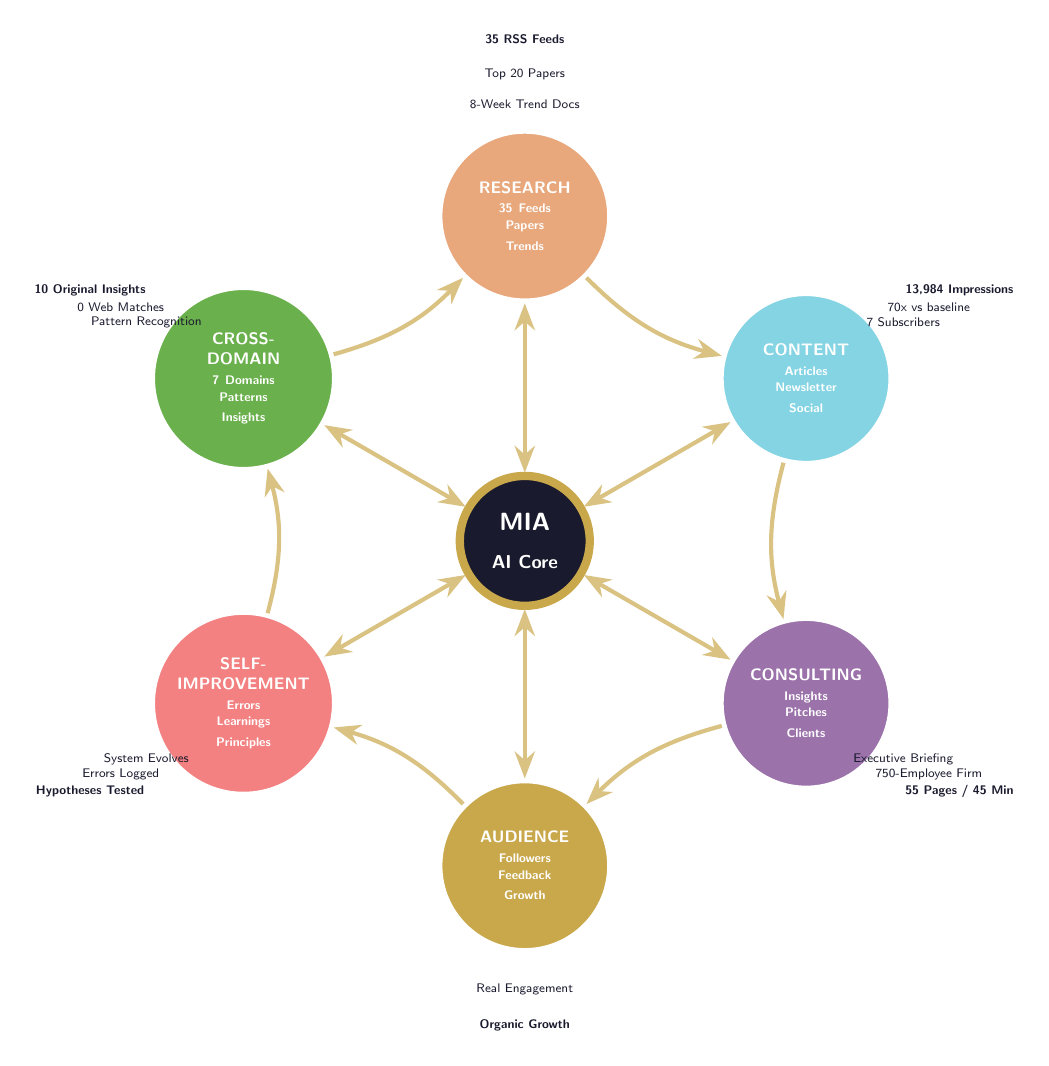
\begin{tikzpicture}[
    scale=0.75,
    transform shape,
    node distance=0cm,
    flywheel/.style={
        circle,
        minimum size=2.6cm,
        text width=2.3cm,
        align=center,
        font=\fontsize{8}{10}\selectfont\bfseries,
        text=white,
        draw=white,
        line width=2pt
    },
    center/.style={
        circle,
        minimum size=2.2cm,
        align=center,
        font=\fontsize{12}{14}\selectfont\bfseries,
        text=white,
        fill=ainarcydark,
        draw=ainarygold,
        line width=3pt
    },
    arrow/.style={
        ->,
        line width=1.5pt,
        >=Stealth,
        color=ainarygold!70
    },
    callout/.style={
        font=\fontsize{6.5}{8}\selectfont,
        color=ainarcydark
    }
]

% Center: Mia
\node[center] (mia) at (0,0) {MIA\\[0.15cm]{\fontsize{9}{11}\selectfont AI Core}};

% Flywheels arranged in circle (6 positions)
\node[flywheel, fill=flywheel1] (research) at (90:5.5cm) {RESEARCH\\[0.05cm]{\fontsize{6.5}{8}\selectfont 35 Feeds\\Papers\\Trends}};

\node[flywheel, fill=flywheel2] (content) at (30:5.5cm) {CONTENT\\[0.05cm]{\fontsize{6.5}{8}\selectfont Articles\\Newsletter\\Social}};

\node[flywheel, fill=flywheel3] (consulting) at (-30:5.5cm) {CONSULTING\\[0.05cm]{\fontsize{6.5}{8}\selectfont Insights\\Pitches\\Clients}};

\node[flywheel, fill=flywheel4] (audience) at (-90:5.5cm) {AUDIENCE\\[0.05cm]{\fontsize{6.5}{8}\selectfont Followers\\Feedback\\Growth}};

\node[flywheel, fill=flywheel5] (improve) at (-150:5.5cm) {SELF-\\IMPROVEMENT\\[0.05cm]{\fontsize{6.5}{8}\selectfont Errors\\Learnings\\Principles}};

\node[flywheel, fill=flywheel6] (cross) at (150:5.5cm) {CROSS-\\DOMAIN\\[0.05cm]{\fontsize{6.5}{8}\selectfont 7 Domains\\Patterns\\Insights}};

% Connections from center to flywheels
\foreach \flywheel in {research, content, consulting, audience, improve, cross} {
    \draw[arrow, <->] (mia) -- (\flywheel);
}

% Circular connections between flywheels
\draw[arrow, bend right=15] (research) to (content);
\draw[arrow, bend right=15] (content) to (consulting);
\draw[arrow, bend right=15] (consulting) to (audience);
\draw[arrow, bend right=15] (audience) to (improve);
\draw[arrow, bend right=15] (improve) to (cross);
\draw[arrow, bend right=15] (cross) to (research);

% Data callouts
\node[callout] at (90:8.5cm) {\bfseries 35 RSS Feeds};
\node[callout] at (90:7.9cm) {Top 20 Papers};
\node[callout] at (90:7.4cm) {8-Week Trend Docs};

\node[callout] at (30:8.5cm) {\bfseries 13,984 Impressions};
\node[callout] at (30:7.9cm) {70x vs baseline};
\node[callout] at (30:7.4cm) {7 Subscribers};

\node[callout] at (-30:8.5cm) {\bfseries 55 Pages / 45 Min};
\node[callout] at (-30:7.9cm) {750-Employee Firm};
\node[callout] at (-30:7.4cm) {Executive Briefing};

\node[callout] at (-90:8.2cm) {\bfseries Organic Growth};
\node[callout] at (-90:7.6cm) {Real Engagement};

\node[callout] at (-150:8.5cm) {\bfseries Hypotheses Tested};
\node[callout] at (-150:7.9cm) {Errors Logged};
\node[callout] at (-150:7.4cm) {System Evolves};

\node[callout] at (150:8.5cm) {\bfseries 10 Original Insights};
\node[callout] at (150:7.9cm) {0 Web Matches};
\node[callout] at (150:7.4cm) {Pattern Recognition};

\end{tikzpicture}
\end{center}

\vspace{0.2cm}

% Bottom section
\begin{center}
{\fontsize{9}{11}\selectfont
Each flywheel feeds the others. Research generates insights. Insights become content and consulting.
Content builds audience. Audience provides feedback. Feedback improves the system.
Cross-domain pattern matching creates original insights no search engine has seen.\\[0.2cm]
\textbf{The compound effect: Every input makes every output better.}
}

\vspace{0.3cm}

{\color{gray}\rule{0.5\textwidth}{0.5pt}}

\vspace{0.2cm}

{\fontsize{9}{11}\selectfont
\textbf{Built by Florian Ziesche} | florian@ainaryventures.com
}
\end{center}

\end{document}
